\section{Experimental Evaluation}
\label{sec:eval}
The experiments examine four questions: (Q1) whether the tested execution
routes retain the records required for each entry path---task, approval,
receipt, and sample links where a task exists---across two configured simulator
scenes and whether each route operates through its bound DAQ and DCW nodes;
(Q2) whether one documented blueprint-onboarding workflow completes on a
fresh application home; (Q3) whether a stale approval context is rejected before
software dispatch; and (Q4) what process samples accompany the tested routes.
These outcomes are kept separate. All plant-facing checks used software
simulators; none involved a physical plant or independent process replication.
Sections~\ref{sec:testbed} to~\ref{sec:coating-onboarding} report the
current-version outcomes; Section~\ref{sec:historical-scenarios} reports the
separate historical optimization record. The evidence is complementary and is
not pooled into a single score.

\subsection{Test Design and Protocol}
\label{sec:eval-protocol}
For a registered task, the integration criterion is a task linked to its
approval, readback-verified receipt, and a run-tagged sample. A direct call has
no task edge; its criterion is a verified receipt/readback and a run-tagged
sample. The fixed-call replay checks record links, not task completion; the
context guard is assessed by whether a changed line, product, recipe, or run is
refused before a driver write. Table~\ref{tab:routes} summarizes the four
studies and their inference limits.

The route-continuity study exercised four entry paths on the v0.8.0
application: registered-harness tasks, a fixed-call harness replay, direct
REST, and a fixture-backed command-line (CLI) task. Two simulator scenes
covered cast film (screw speed over OPC UA; thickness over MQTT; target
48--52\,$\mu$m) and continuous annealing (zone-3 setpoint and strip
temperature over Modbus TCP; target 700--760\,$^{\circ}$C). Each scene
blueprint declared its DAQ and DCW nodes, and the route configuration bound the
agent and channel tool catalog to those nodes; the recorded reads and writes
used the bound thickness/screw-speed and strip-temperature/zone-3 nodes. The
registered-harness path ran three sequential tasks per scene on one persistent
simulator; the registered adapter used a fixed cloud model
(\texttt{glm-5.3-flash}) with a three-value prevalidated set per control. Each
task used its own production and task context, while process state carried
forward. After each verified receipt, the runner waited 20\,s, probed and
ingested one sample, queried it by active-run ID, and then checked task state,
so the completion-to-sample latency was not recorded. The fixed-call replay,
direct REST call, and CLI task ran once per scene in separate isolated
environments.

The production MQTT queue and Timescale service were not used in the
route-study runs; R22 ran isolated with an in-process queue and SQLite storage.
Each sample was a single explicit driver probe stored and
queried through the local SQLite fallback with online DAQ collection disabled;
the route results therefore assess invocation and application-record handling,
not the online DAQ pipeline. Fixture-backed routes used deterministic input;
direct REST created no task and did not invoke an external model. All
route-study approvals were synthetic administrator decisions.

A separate v0.8.3 onboarding replay used a fresh isolated application home and
the documented C01 blueprint. The blueprint configured one Modbus/TCP device
with four DCW setpoints and seven DAQ nodes, plus MES REST scalar, 48-point
vector, table, and image forms. Channel construction bound the agent and tool
catalog to those nodes. Dedicated local MQTT and Timescale services were online
for DAQ checks; object storage was unavailable, so image artifacts used the
local-disk fallback. This was one configuration replay, not a route-study
trial.

The approval-context suite changed one field of the approved
line--product--recipe--run tuple at a time for recipe apply, trial, and rollback
with dispatch enabled: four fields for each of the three operations. A separate
fault-injection case changed context after asynchronous grant revalidation but
before the caller's final synchronous check. A test-only ablation removed only
the tuple comparison while retaining the other checks. These outcomes were
recorded in mock-driver state and are not process-level reliability estimates.

\begin{table}[!t]
\centering
\caption{Experiment matrix. All entries are software-level checks, not
independent process replications.}
\label{tab:routes}
\footnotesize
\setlength{\tabcolsep}{3pt}
\begin{tabularx}{\columnwidth}{@{}>{\raggedright\arraybackslash}p{1.55cm}X@{}}
\toprule
Study & Design, observed result, and inference limit \\
\midrule
Route continuity and binding (Q1) &
Four entry paths in two simulator scenes; each route bound to the scene's DAQ
and DCW nodes. Six model-mediated registered tasks verified task, approval,
receipt, and sample links; all route samples were below target. One 20-s sample
per task or call (12 total); no unbound-node negative test. \\
C01 onboarding and binding (Q2) &
One documented blueprint: four DCW setpoints, seven DAQ nodes, four MES forms.
Preflight, provisioning, channel construction, and the V1--V6 verifier
completed; one 37--39\,m/min simulator-confirmed write. One blueprint;
unpinned build. \\
Approval context (Q3) &
Four tuple fields for each of three recipe operations with dispatch enabled;
one queued between-check mutation. Every injected one-field change was blocked
before a mock write; an ablation that removed only the tuple comparison admitted
six product/run changes. Mock state only. \\
Archived optimization (historical) &
Four seed-42 scripted direct-node missions, one trajectory each. Terminal
readings were in band; requests are not device readbacks. Not current-route or
repeatability evidence. \\
\bottomrule
\end{tabularx}
\end{table}

\subsection{Route Results and Node Bindings}
\label{sec:testbed}
All six model-mediated registered tasks completed, and their task, approval,
receipt, and sample links were verified. Cast-film settings of
125/130/125\,rpm produced single 20-s samples of
45.69/46.69/45.69\,$\mu$m; annealing settings of 745\,$^{\circ}$C produced
679.60/677.70/678.10\,$^{\circ}$C. Pre-task values were
55.82/45.69/46.69\,$\mu$m and 675.40/678.30/676.90\,$^{\circ}$C, so five tasks
started below their band and one above. The post-trial samples therefore
reflect carried-over state and a single 20-s probe; they do not describe a
response trajectory, steady state, or the quality of the model-selected
settings. The recorded reads and writes used the bound thickness/screw-speed
and strip-temperature/zone-3 nodes. The study did not inject an unbound-node
request, so binding is observed as the precondition under which the routes
succeeded, not as an ablated factor.

The remaining three routes met their record criteria but differed in task
linkage and model involvement. The fixed-call replay linked both tasks to
approval, receipt, and active-run samples without asserting task completion;
its samples were 46.37\,$\mu$m and 674.80\,$^{\circ}$C. Direct REST returned
verified receipts/readbacks and run-tagged samples; its samples were
46.37\,$\mu$m and 675.20\,$^{\circ}$C. The fixture-backed CLI task completed
both tasks and linked their samples; its samples were 46.38\,$\mu$m and
674.40\,$^{\circ}$C. All three used 125\,rpm and 735\,$^{\circ}$C, whereas the
registered runs used 745\,$^{\circ}$C. The cast-film samples are similar across
routes; the annealing samples differ by roughly 4--5\,$^{\circ}$C, consistent
with the setpoint difference. These similarities are consistent with a shared
handler, but separate environments and one sample per task or call do not
establish route equivalence, process attainment, or reuse across scenes.

\subsection{HITL Approval Context and Stale-Context Rejection (Mock State)}
\label{sec:guard-results}
For a recipe write, the handler checks the bound recipe, active run, candidate
parameters, and route timing; if human-in-the-loop (HITL) approval is required,
it creates a card binding the actor, operation, candidate values, applicable
limits, expiry (30\,min for recipe dispatch; 180\,s for single-parameter HITL),
and the active tuple. After approval, the handler
rechecks authority and grant, compares the current tuple with the approved
tuple, and only then enters DCW dispatch. The queued context change was
refused at the same comparison.

The production handler blocked every injected one-field mutation before a mock
write or execution record, and the queued change was refused before
\texttt{recipe\_apply} dispatch. In the ablation, removing the tuple comparison
allowed six product/run changes through; each produced two mock writes and an
execution record, while the other checks still blocked line/recipe changes.
The comparison is therefore the decisive check for product/run identity,
whereas the other checks cover line and recipe changes.

The study is mock-state only. It does not demonstrate atomicity during network
or device I/O, safe physical operation, operator effectiveness, or human-review
performance. Synthetic approval also does not measure approval latency or
error rates.

\begin{figure*}[!t]
\centering
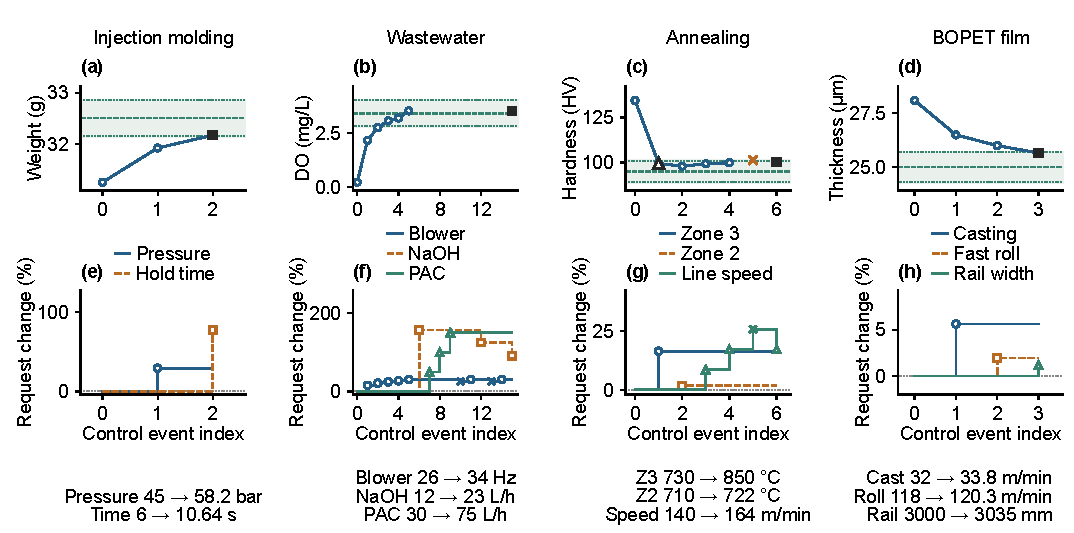
\includegraphics[width=\textwidth]{resources/fig-missions-controls.pdf}
\caption{Archived optimization records for four simulator scenarios (seed 42;
one scripted trajectory per scenario). Upper panels show process-variable (PV)
observations with scenario-specific target bands; lower panels show requested
setpoint changes as percentages of each baseline, and event indices give order,
not elapsed time. Bottom annotations give the first and last requested values.
Black squares mark mission-final readings; for injection molding and BOPET they
overlap the last observation. In wastewater treatment, later NaOH and PAC
requests belong to pH and total-phosphorus stages, and the mission-final DO
reading (3.50\,mg/L) is not joined to the last trajectory observation
(3.517\,mg/L). Crosses mark reverted requests. In annealing, the open triangle
is the 99.46-HV event without a linked optimization record; the cross is the
101.3-HV event-text value after a reverted 176\,m/min candidate, not a
structured trajectory observation. Requests are not device readbacks. These
historical direct-node missions are separate from the route study and do not
show current route performance or a common optimizer score.}
\label{fig:missions}
\end{figure*}

\subsection{Blueprint Onboarding and DAQ/DCW Binding}
\label{sec:coating-onboarding}
The C01 blueprint instantiated the documented coating line from configuration
objects: one Modbus/TCP device with four DCW
setpoints and seven DAQ nodes, plus MES REST scalar, 48-point vector, table, and
image forms. Channel construction bound the agent and tool catalog to those
nodes. Its connectivity preflight, line provisioning, and channel construction
completed with the expected objects and no failures, and all four MES forms
returned records with the expected format and field dictionary. The V1--V6
verifier confirmed sample availability for all seven DAQ nodes, range
rejection, legal write/readback, recipe mapping, channel/plugin checks, and zero
writes to a protected demonstration line.

One smoke proposal used the test-only automatic-approval policy to change line
speed from 37 to 39\,m/min within the 28--48\,m/min recipe window; the PLC twin
confirmed the write. The approval was synthetic. The replay ran on a
working-tree build whose source commit was not pinned, and it did not vary the
profile or binding set between runs. These checks therefore establish one
documented blueprint-to-simulator onboarding instance, not human-review
performance, film quality, process attainment, arbitrary protocol coverage,
configuration reuse, repeatability, or physical transfer. Supplementary
File~S1 includes the inputs, health and DAQ status, runner output, and complete
V1--V6 log.

\subsection{Archived Optimization Execution Records}
\label{sec:historical-scenarios}
The current route study collected one post-trial process sample per task or
call.
Fig.~\ref{fig:missions} instead shows four archived seed-42 optimization
missions from an earlier scripted direct-node interface. Each mission iterates:
observe the process variable, request a bounded setpoint change, apply it
through the direct node, and observe the next process variable. The event index
gives order, not elapsed time. The upper row plots observations against each
scenario's target band; the lower row plots requested changes as percentages of
each baseline; the annotations give the first and last requested values.

In injection molding, hold pressure and time increased from 45 to
58.2\,bar and 6 to 10.64\,s; measured weight rose from 31.25 to 32.17\,g,
ending 0.02\,g inside the $32.5\pm0.35$\,g window. Five wastewater blower
increments from 26 to 34\,Hz raised dissolved oxygen (DO) from 0.214 to
3.517\,mg/L, inside the $3.4\pm0.6$\,mg/L window; later NaOH and
polyaluminium chloride (PAC) requests moved from 12 to 23\,L/h and 30 to
75\,L/h in separate pH and phosphorus stages. In annealing, the zone-3 request
rose from 730 to 850\,$^{\circ}$C without a linked optimization record; zone-2
moved from 710 to 722\,$^{\circ}$C and line speed from 140 to
164\,m/min, producing 97.88--99.84 Vickers hardness (HV), and the terminal
value was 100.08\,HV in the $95\pm6$\,HV window. For biaxially oriented
polyethylene terephthalate (BOPET) film, casting speed, fast-roll speed, and
rail width changed from 32 to 33.8\,m/min, 118 to 120.3\,m/min, and 3000 to
3035\,mm; thickness fell from 28.10 to 25.66\,$\mu$m, ending
0.04\,$\mu$m inside the upper edge of its $25.0\pm0.7$\,$\mu$m window.

These archived records illustrate scenario-specific feedback, not
repeatability or current-route attainment. They also show that the archived
scenarios can reach in-band terminal readings under scripted direct-node
control, but they measure different process variables from the route study and
do not bound the route's cast-film thickness or annealing strip temperature.
The historical missions are not pooled with the route results.

\FloatBarrier

\subsection{Evidence Synthesis}
The route study answers Q1 and Q4: across two preconfigured mappings, every
tested task and direct-call contract retained its required records, every route
used its bound DAQ and DCW nodes, and every route-linked sample was below
target. The onboarding replay answers Q2: the documented C01 configuration
completed on a fresh application home, produced the expected objects with
isolated online MQTT/Timescale, and confirmed one simulator write. The
mock-state comparison answers Q3: the tested context check blocked stale
requests before software dispatch. Fig.~\ref{fig:missions} is historical
optimization evidence and is not pooled with these results.

Together, these results distinguish command completion from process outcome:
a verified readback confirms the setpoint path, whereas the later run-tagged
sample indicates whether the process variable was inside its target band at
the probe instant. The study establishes record linkage across the tested entry
paths, that the routes used their configured bindings, stale-context rejection
in mock state, and one simulated onboarding instance; it does not establish
process improvement, general portability, or physical-plant performance. Supplementary File~S1 includes the route inputs
and logs, onboarding replay, historical records, and evidence/hash manifests.
The model-mediated tasks are not deterministic replays, and the route samples
are not independent replicates.
